\documentclass{article}
\usepackage[T1]{fontenc}
\usepackage{lmodern}
\usepackage{graphicx}
\usepackage{amsmath,amssymb}
\usepackage[a4paper,margin=2cm]{geometry}
\usepackage[absolute,overlay]{textpos}
\setlength{\TPHorizModule}{1mm}
\setlength{\TPVertModule}{1mm}
\usepackage[indonesian]{babel}
\usepackage{hyperref}
\setlength{\emergencystretch}{2em}
% unit: Halaman 31

\begin{document}

% === Halaman 31 (python/native) ===

Ri – 1 = Li 





Li – 1 = Ri  f(Ri – 1, Ki) = Ri  f(Li, Ki)

Dekripsi:

31

% deskripsi: gambar native xref 154
\noindent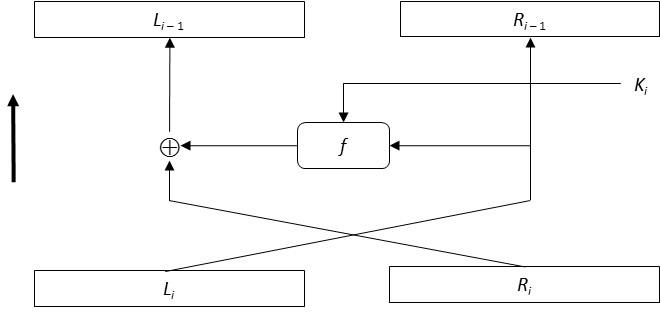
\includegraphics[width=0.85\textwidth]{../../images/python/page_031_img_01.jpeg}

\end{document}
